%--------------------------------------------------------------------------------------
% Thesis 1. paper
% Author: Gabor Szarnyas
% Created at: May 2013
%--------------------------------------------------------------------------------------


%--------------------------------------------------------------------------------------
% Page format
%--------------------------------------------------------------------------------------
\documentclass[12pt,a4paper,twoside]{report}           
%\documentclass[10pt,a4paper,twoside,openright]{report}  


%--------------------------------------------------------------------------------------
% Package incudes
%--------------------------------------------------------------------------------------
\usepackage{t1enc} 
\usepackage[utf8]{inputenc}
\usepackage{amsmath}
\usepackage{amssymb}
\usepackage{enumerate}
\usepackage[thmmarks]{ntheorem}
\usepackage{graphicx}
\usepackage{epsfig}
\usepackage{listings}
\usepackage{color} 
\usepackage{lastpage}
\usepackage{anysize}
\usepackage{longtable}
\usepackage[english]{babel}
\usepackage{sectsty}
\usepackage{setspace}
\usepackage[hang]{caption}
\usepackage{hyperref}
\usepackage{tabularx}
%\usepackage{times}
%\usepackage{libertine-type1}
\usepackage{hyphenat}
\usepackage{enumitem}
\usepackage{inconsolata} % typewriter 
\usepackage{subcaption}
\usepackage{todonotes}
\usepackage{fourier} % changed Times to Fourier


%--------------------------------------------------------------------------------------
% Custom commands
%--------------------------------------------------------------------------------------
% insert pictures
\newcommand{\pic}[2]{
\begin{figure}[htb]
   \center   
   \caption{#2}
   \label{fig:#1}  
      \includegraphics{figures/#1}
\end{figure}
}

% insert and resize picture to the width of the screen
\newcommand{\picr}[2]{
\begin{figure}[htb]
   \center   
   \caption{#2}
   \label{fig:#1}  
     \resizebox{\linewidth}{!}{
      \includegraphics{figures/#1}
      } 
\end{figure}
}


\newcommand{\picfifty}[2]{
\begin{figure}[htb]
   \center
   \caption{#2}
   \label{fig:#1}
     \resizebox{0.5\linewidth}{!}{
      \includegraphics{figures/#1}
      }
\end{figure}
}

\newcommand{\picseventy}[2]{
\begin{figure}[htb]
   \center
   \caption{#2}
   \label{fig:#1}
     \resizebox{0.7\linewidth}{!}{
      \includegraphics{figures/#1}
      }
\end{figure}
}

% insert tables
% 1. param�ter: caption
% 2. param�ter: label
% 3. param�ter: oszlopok definiálása
\newenvironment*{tabl}[3]{
   \begin{table}[htb]
   
   \caption{#1}
   \label{tab:#2}
   \centering
   \begin{tabular}{#3}
}{
   \end{tabular}
   \end{table}
}


\newcommand{\figref}[1]{Figure~\autoref{fig:#1}}                      
\newcommand{\secref}[1]{section~\ref{sect#1}}
% section reference \newcommand{\code}[1]{{\upshape\ttfamily\scriptsize\indent #1}} % formatted code
\newcommand{\code}[1]{{\small \texttt{#1}}} % formatted code
\newcommand{\tool}[1]{\texttt{#1}}
%--------------------------------------------------------------------------------------
% Constant strings
%--------------------------------------------------------------------------------------
\newcommand{\pauthor}{G\'abor Sz\'arnyas}
\newcommand{\psvisor}{Dr.~Istv\'an R\'ath, Dr.~D\'aniel Varr\'o}
\newcommand{\ptitle}{Superscalable modeling}
\newcommand{\pdep}{Department of Measurement and Information Systems}
\newcommand{\ptype}{Scientific Students' Associations Report}
\newcommand{\ptool}{Dependency Analysis Tool}

%\newcommand{\todo}[1]{\textbf{TODO: }{#1}}

\newcommand{\sectref}[1]{section~\aref{sect:#1}}

%--------------------------------------------------------------------------------------
% Declarations
%--------------------------------------------------------------------------------------
\DeclareMathOperator*{\argmax}{arg\,max}
%\DeclareMathOperator*[1]{\floor}{arg\,max}
\DeclareMathOperator{\sign}{sgn}
\DeclareMathOperator{\rot}{rot}
\definecolor{lightgray}{rgb}{0.95,0.95,0.95}
 
\author{\pauthor}
\title{\ptitle}



%--------------------------------------------------------------------------------------
% Page layout setup
%--------------------------------------------------------------------------------------
% we need to redefine the pagestyle plain
% another possibility is to use the body of this command without \fancypagestyle
% and use \pagestyle{fancy} but in that case the special pages
% (like the ToC, the References, and the Chapter pages)remain in plane style

\pagestyle{plain}
%\setlength{\parindent}{0pt}                  % more clear; in english documents
%\setlength{\parskip}{8pt plus 3pt minus 3pt} % more clear; in english documents
\setlength{\parindent}{12pt}                  % in hungarian documents
\setlength{\parskip}{0pt}                     % in hungarian documents
\marginsize{35mm}{25mm}{15mm}{15mm}           % anysize package
\setcounter{secnumdepth}{0}
\sectionfont{\large\upshape\bfseries}
\setcounter{secnumdepth}{2}
\singlespacing{}
\frenchspacing{}
%\setlist[description]{leftmargin=0em}                      % remove indent from descriptions
\setitemize{noitemsep,topsep=0pt,parsep=0pt,partopsep=0pt}  % compact list

%--------------------------------------------------------------------------------------
%	Setup hyperref package
%--------------------------------------------------------------------------------------
\hypersetup{
    %bookmarks=true,           % show bookmarks bar?
    unicode=false,             % non-Latin characters in Acrobat’s bookmarks
    pdftitle={\ptitle},        % title
    pdfauthor={\pauthor},      % author
    pdfsubject={\ptype},       % subject of the document
    pdfcreator={\pauthor},     % creator of the document
    pdfproducer={Producer},    % producer of the document
    pdfkeywords={keywords},    % list of keywords
    pdfnewwindow=true,         % links in new window
    colorlinks=true,           % false: boxed links; true: colored links
    linkcolor=black,           % color of internal links
    citecolor=black,           % color of links to bibliography
    filecolor=black,           % color of file links
    urlcolor=black             % color of external links
}


%--------------------------------------------------------------------------------------
% Set up listings
%--------------------------------------------------------------------------------------
% \lstset{
% 	basicstyle=\scriptsize\ttfamily,              % print whole listing small
% 	keywordstyle=\color{black}\bfseries\underbar, % underlined bold black keywords
% 	identifierstyle=, 					          % nothing happens
% 	commentstyle=\color{white},                   % white comments
% 	stringstyle=\scriptsize\sffamily, 			  % typewriter type for strings
% 	showstringspaces=false,                       % no special string spaces
% 	aboveskip=3pt,
% 	belowskip=3pt,
% 	columns=fixed,
% 	backgroundcolor=\color{lightgray},
% } 		
%\def\lstlistingname{lista}	

% standard IncQuery stuff
\usepackage{color}
\definecolor{listinggray}{rgb}{0.9,0.9,0.9}
\definecolor{keywordcolor}{rgb}{0.5,0,0.1}
\definecolor{commentcolor}{rgb}{0,0.3,0.1}
\definecolor{stringcolor}{rgb}{0,0,1}
\usepackage{listings}
\lstdefinelanguage{viatra}
{morekeywords={@Interpretation,@Trigger,package,private,count,sum,max,min,avg,shareable,trigger,guard,eval,
asmfunction,rule,gtrule,if,do,choose,forall,iterate,print,println,log,apply,
    entity,relation,supertypeOf,subtypeOf,typeOf,instanceOf,try,else,pattern,
    precondition,postcondition,action,neg,find,import,namespace,in,below,out,
    inout,let,multiplicity,many_to_one,many_to_many,one_to_many,one_to_one,
    isAggregation,inverse,seq,update,ref,true,false,call,machine,or,
    undef,rename,new,del,delete,move,copy,value,interface,class,,setFrom,setTo,with,when,check,change,appear,disappear,cdrule,transformation,common,from,to,toInteger},
    sensitive=true, morecomment=[l]{//}, morecomment=[s]{/*}{*/}, morestring=[b]{"}, }
\lstset{backgroundcolor=\color{listinggray}}
\lstset{basicstyle=\scriptsize\ttfamily}
\lstset{commentstyle=\itshape\color{commentcolor}\ttfamily}
\lstset{stringstyle=\color{stringcolor}\ttfamily}
\lstset{frameround=tttt}
\lstset{captionpos=b}
\lstset{keywordstyle=\color{keywordcolor}\bfseries\ttfamily}
\lstset{showstringspaces=false}
\lstset{tabsize=2}
\lstset{numbers=left,numberstyle=\scriptsize\ttfamily,stepnumber=1,numbersep=5pt}
\lstset{language=viatra}
\lstset{escapeinside={(*@}{@*)}}


%--------------------------------------------------------------------------------------
% Setup captions
%--------------------------------------------------------------------------------------
\captionsetup[figure]{
%labelsep=none,
%font={footnotesize,it},
%justification=justified,
width=.75\textwidth,
aboveskip=10pt}

\renewcommand{\captionlabelfont}{\small\bf}
\renewcommand{\captionfont}{\footnotesize\it}

\newcommand{\tss}{\textsuperscript}

\newcommand{\incquery}{\textsc{EMF-IncQuery}}
\newcommand{\incqueryD}{\textsc{IncQuery-D}}

\sloppy

%--------------------------------------------------------------------------------------
% Main document content
%--------------------------------------------------------------------------------------
\begin{document}

\pagenumbering{arabic}
\onehalfspacing

%--------------------------------------------------------------------------------------
%	The title page
%--------------------------------------------------------------------------------------
\begin{titlepage}
\begin{center}
%\includegraphics[width=60mm,keepaspectratio]{figures/BMElogo.png}\\

\includegraphics[width=60mm,keepaspectratio]{figures/BME1782nagy.pdf}\\
\vspace{0.3cm}
\textbf{Budapest University of Technology and Economics}\\
\textmd{Faculty of Electrical Engineering and Informatics}\\
\textmd{\pdep}\\[5cm]
 
\vspace{0.4cm}
{\huge \bfseries \ptitle}\\[0.8cm]
\vspace{0.5cm}
\textsc{\Large \ptype}\\[4cm]

\begin{tabular}{cc}
 \makebox[7cm]{\emph{Author}} & \makebox[7cm]{\emph{Supervisors}} \\
 \makebox[7cm]{\pauthor} & \makebox[7cm]{\psvisor}
\end{tabular}

\vfill
{\large \today}
%{\large October 26, 2012}
\end{center}
\end{titlepage}

~
\vfill
\clearpage

       % title		+ blank
\emph{I would like to thank to my supervisors István Ráth, Bence Izsó and Dániel Varró. I also wish to thank G\'abor Berg\-mann for the help with the adaptation of the Rete implementation of \eiq.}

\emph{I also would like to thank my family for their constant support.} \vfill \clearpage

\begin{center}
\large
\textbf{HALLGATÓI NYILATKOZAT}\\
\end{center}

Alulírott \emph{Szárnyas Gábor}, szigorló hallgató kijelentem, hogy ezt a diplomatervet meg nem engedett segítség nélkül, saját magam készítettem, csak a megadott forrásokat (szakirodalom, eszközök stb.) használtam fel. Minden olyan részt, melyet szó szerint, vagy azonos értelemben, de átfogalmazva más forrásból átvettem, egyértelműen, a forrás megadásával megjelöltem.

Hozzájárulok, hogy a jelen munkám alapadatait (szerző(k), cím, angol és magyar nyel\-vű tartalmi kivonat, készítés éve, konzulens(ek) neve) a BME VIK nyilvánosan hozzáférhető elektronikus formában, a munka teljes szövegét pedig az egyetem belső hálózatán keresztül (vagy autentikált felhasználók számára) közzétegye. Kijelentem, hogy a benyújtott munka és annak elektronikus verziója megegyezik.

\begin{flushleft}
\vspace*{1cm}
Budapest, 2013. május 23.
\end{flushleft}

\begin{flushright}
 \vspace*{1cm}
 \makebox[7cm]{\rule{6cm}{.4pt}}\\
 \makebox[7cm]{\emph{Szárnyas Gábor}}\\
 \makebox[7cm]{hallgató}
\end{flushright}
\thispagestyle{empty}

\vfill
\clearpage
\thispagestyle{empty} % an empty page
 % thanks		+ declaration 
% %----------------------------------------------------------------------------
% % Abstract in Hungarian
% %----------------------------------------------------------------------------
% \chapter*{Kivonat}\addcontentsline{toc}{chapter}{Abstract in Hungarian}
% 
% Az adatintenzív alkalmazások nagy kihívása a lekérdezések hatékony kiértékelése. A modellvezérelt szoftvertervezés (MDE) során az eszközök és a transzformációk különböző bonyolultságú lekérdezéssekkel dolgoznak. Míg a szoftvermodellek mérete és komplexitása folyamatosan nő, a hagyományos MDE eszközök gyakran nem skálázódnak megfelelően, így csökkentve a fejlesztés produktivitását és növelve a költségeket.
% 
% Ugyan az újgenerációs, ún. NoSQL adatbázis-kezelő rendszerek többsége képes horizontális skálázhatóságra, az ad-hoc lekérdezéseket nem támogatja olyan hatékonyan, mint a relációs adatbázisok. Mivel a modellvezérelt alkalmazások tipikusan komplex lekérdezéseket futtatnak, a NoSQL adatbázis-kezelők közvetlenül nem használhatók ilyen célra.
% 
% Diplomatervem célja, hogy az \eiq{}-ben alkalmazott inkrementális gráfmintaillesztő algoritmust elosztott, felhőalapú infrastruktúrára implementáljam. Az \iqd{} prototípus skálázható, így képes több számítógépből álló fürtön nagy modelleket kezelni és komplex lekérdezések hatékonyan kiértékelni. Az elképzelés életképességét előzetes mérési eredményeink igazolják.
% 
% \vfill

%----------------------------------------------------------------------------
% Abstract in English
%----------------------------------------------------------------------------
\chapter*{Abstract}\addcontentsline{toc}{chapter}{Abstract in English}

Queries are the foundations of data intensive applications. In model-driven software engineering (MDE), model queries are core technologies of tools and transformations. As software models are rapidly increasing in size and complexity, traditional MDE tools frequently exhibit scalability issues that decrease productivity and increase costs.

While such scalability challenges are a constantly hot topic in the database community and recent efforts of the NoSQL movement have partially addressed many shortcomings, this happened at the cost of sacrificing the powerful ad-hoc query capabilities of SQL. Unfortunately, this is a critical problem for MDE applications, as their queries can be significantly more complex than in general database applications.

In my thesis work, I aim to address this challenge by adapting incremental graph search techniques -- known from the \eiq{} framework -- to the distributed cloud infrastructure. \iqd, my prototype system can scale up from a single-node tool to a cluster of nodes that can handle very large models and complex queries efficiently. The feasibility of my approach is supported by early experimental results.

\vfill
    % abstract hu + abstract en
\tableofcontents      % toc

\chapter{Introduction}

\section{Introduction}
\label{sec:intro}

% Queries in MDE: scalability challenge
Nowadays, model-driven software engineering (MDE) plays an important role in the development processes of critical embedded systems. Advanced modeling tools provide support for a wide range of development tasks such as requirements and traceability management, system modeling, early design validation, automated code generation, model-based testing and other validation and verification tasks. 
With the dramatic increase in complexity that is also affecting critical embedded systems in recent years, modeling toolchains are facing scalability challenges as the size of design models constantly increases, and automated tool features become more sophisticated.

% The role/importance  of expressive and incremental queries in MDE
Many scalability issues can be addressed by improving query performance. \emph{Incremental evaluation} of model queries aims to reduce query response time by limiting the impact of model modifications to query result calculation. Such algorithms work by either (i) building a cache of interim query results and keeping it up-to-date as models change (e.g.\ \eiq{}~\cite{models10}) or (ii) applying impact analysis techniques and re-evaluating queries only in contexts that are affected by a change (e.g.\ the Eclipse OCL Impact Analyzer~\cite{OCLIA}). This technique has been proven to improve performance dramatically in several scenarios (e.g.\ on-the-fly well-formedness validation or model synchronization), at the cost of increasing memory consumption. Unfortunately, this overhead is combined with the increase in model sizes due to in-memory representation (found in state-of-the-art frameworks such as EMF~\cite{EMF}). Since single-computer heaps cannot grow arbitrarily (as response times degrade drastically due to garbage collection problems), memory consumption is the most significant scalability limitation.% of the single workstation architecture.


% Scalability for databases and linked data
% graph databases, RDF/SPARQL
% at the cost of expressive ad-hoc queries

An alternative approach to tackling MDE scalability issues is to make use of advances in persistence technology. As the majority of model-based tools uses a graph-oriented data model, recent results of the NoSQL and Linked Data movement~\cite{neo4j,openvirtuoso,sesame} are straightforward candidates for adaptation to MDE purposes. Unfortunately, this idea poses difficult conceptual and technological challenges: (i) property graph databases lack strong metamodeling support and their query features are simplistic compared to MDE needs, and (ii) the underlying data representation format of semantic databases (RDF~\cite{website:rdf_standard}) has crucial conceptual and technological differences to traditional metamodeling languages such as Ecore~\cite{EMF}. Additionally, while there are initial efforts to overcome the mapping issues between the MDE and Linked Data worlds~\cite{hillairet2008bridging}, even the most sophisticated NoSQL storage technologies lack efficient and mature support for executing expressive queries incrementally.

% Goals: scale up to large models, yet maintain scalability for expressive and incremental queries
% proposal, prototype tool
% engineering principles: adaptability
% initial feasibility and performance evaluation experiments

We aim to address these challenges by adapting incremental graph search techniques from \eiq{} to the cloud infrastructure. We introduce \iqd, a prototype system based on a distributed Rete network~\cite{Forgy} that can scale up from a single-workstation tool to a cluster to handle very large models and complex queries efficiently (\autoref{sec:overview}). We carry out an initial performance evaluation in the context of on-the-fly well-formedness validation of software design models (\autoref{sec:evaluation}), discuss related work in \autoref{sec:relwork} and conclude the thesis in \autoref{sec:conclusion}.

\begin{figure}
\begin{center}
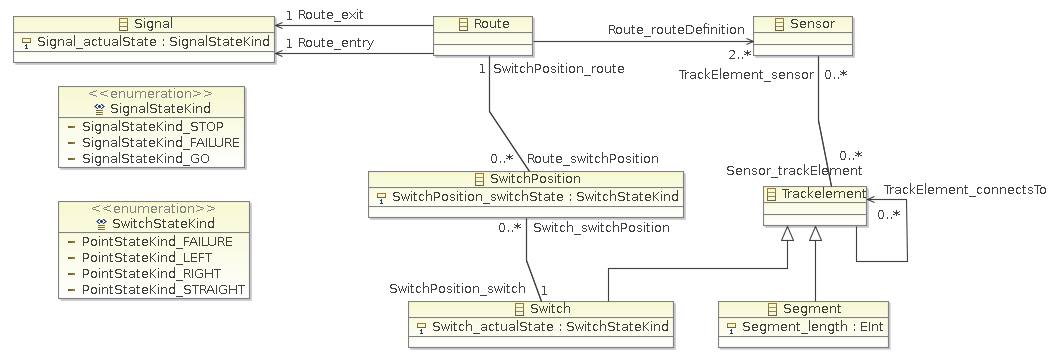
\includegraphics[]{figures/TrainMetamodel}
\caption{}
\label{fig:}
\end{center}
\end{figure}

 
\section{Overview of the Approach}
\label{sec:overview}

The primary goal of our proposal is to provide a scalable architecture for executing incremental queries over large models.  Our approach is based on the following foundations: (i) a distributed model storage system that (ii) supports a graph-oriented data representation format, and (iii) a graph query language (adapted from the \incquery{} framework). The novel contribution of this paper is an architecture that consists of a (i) distributed model management middleware, and a (ii) distributed and stateful pattern matcher network based on the Rete algorithm. \incqueryD{} provides incremental query execution by \emph{indexing model contents} and \emph{capturing model manipulation operations} in the middleware layer, and \emph{propagating change tokens} along the pattern matcher network to \emph{produce query results and query result changes} (corresponding to model manipulation transactions) efficiently. As the primary sources of memory consumption, i.e.\ both the indexing and intermediate Rete nodes can be distributed in a cloud infrastructure, the system is expected to scale well beyond the limitations of the traditional single workstation setup.

\subsection{Architecture}
\label{architecture}
The \incqueryD{} architecture in an example configuration scenario is shown in \autoref{fig:architecture}.

\begin{figure}[!t]
\begin{center}
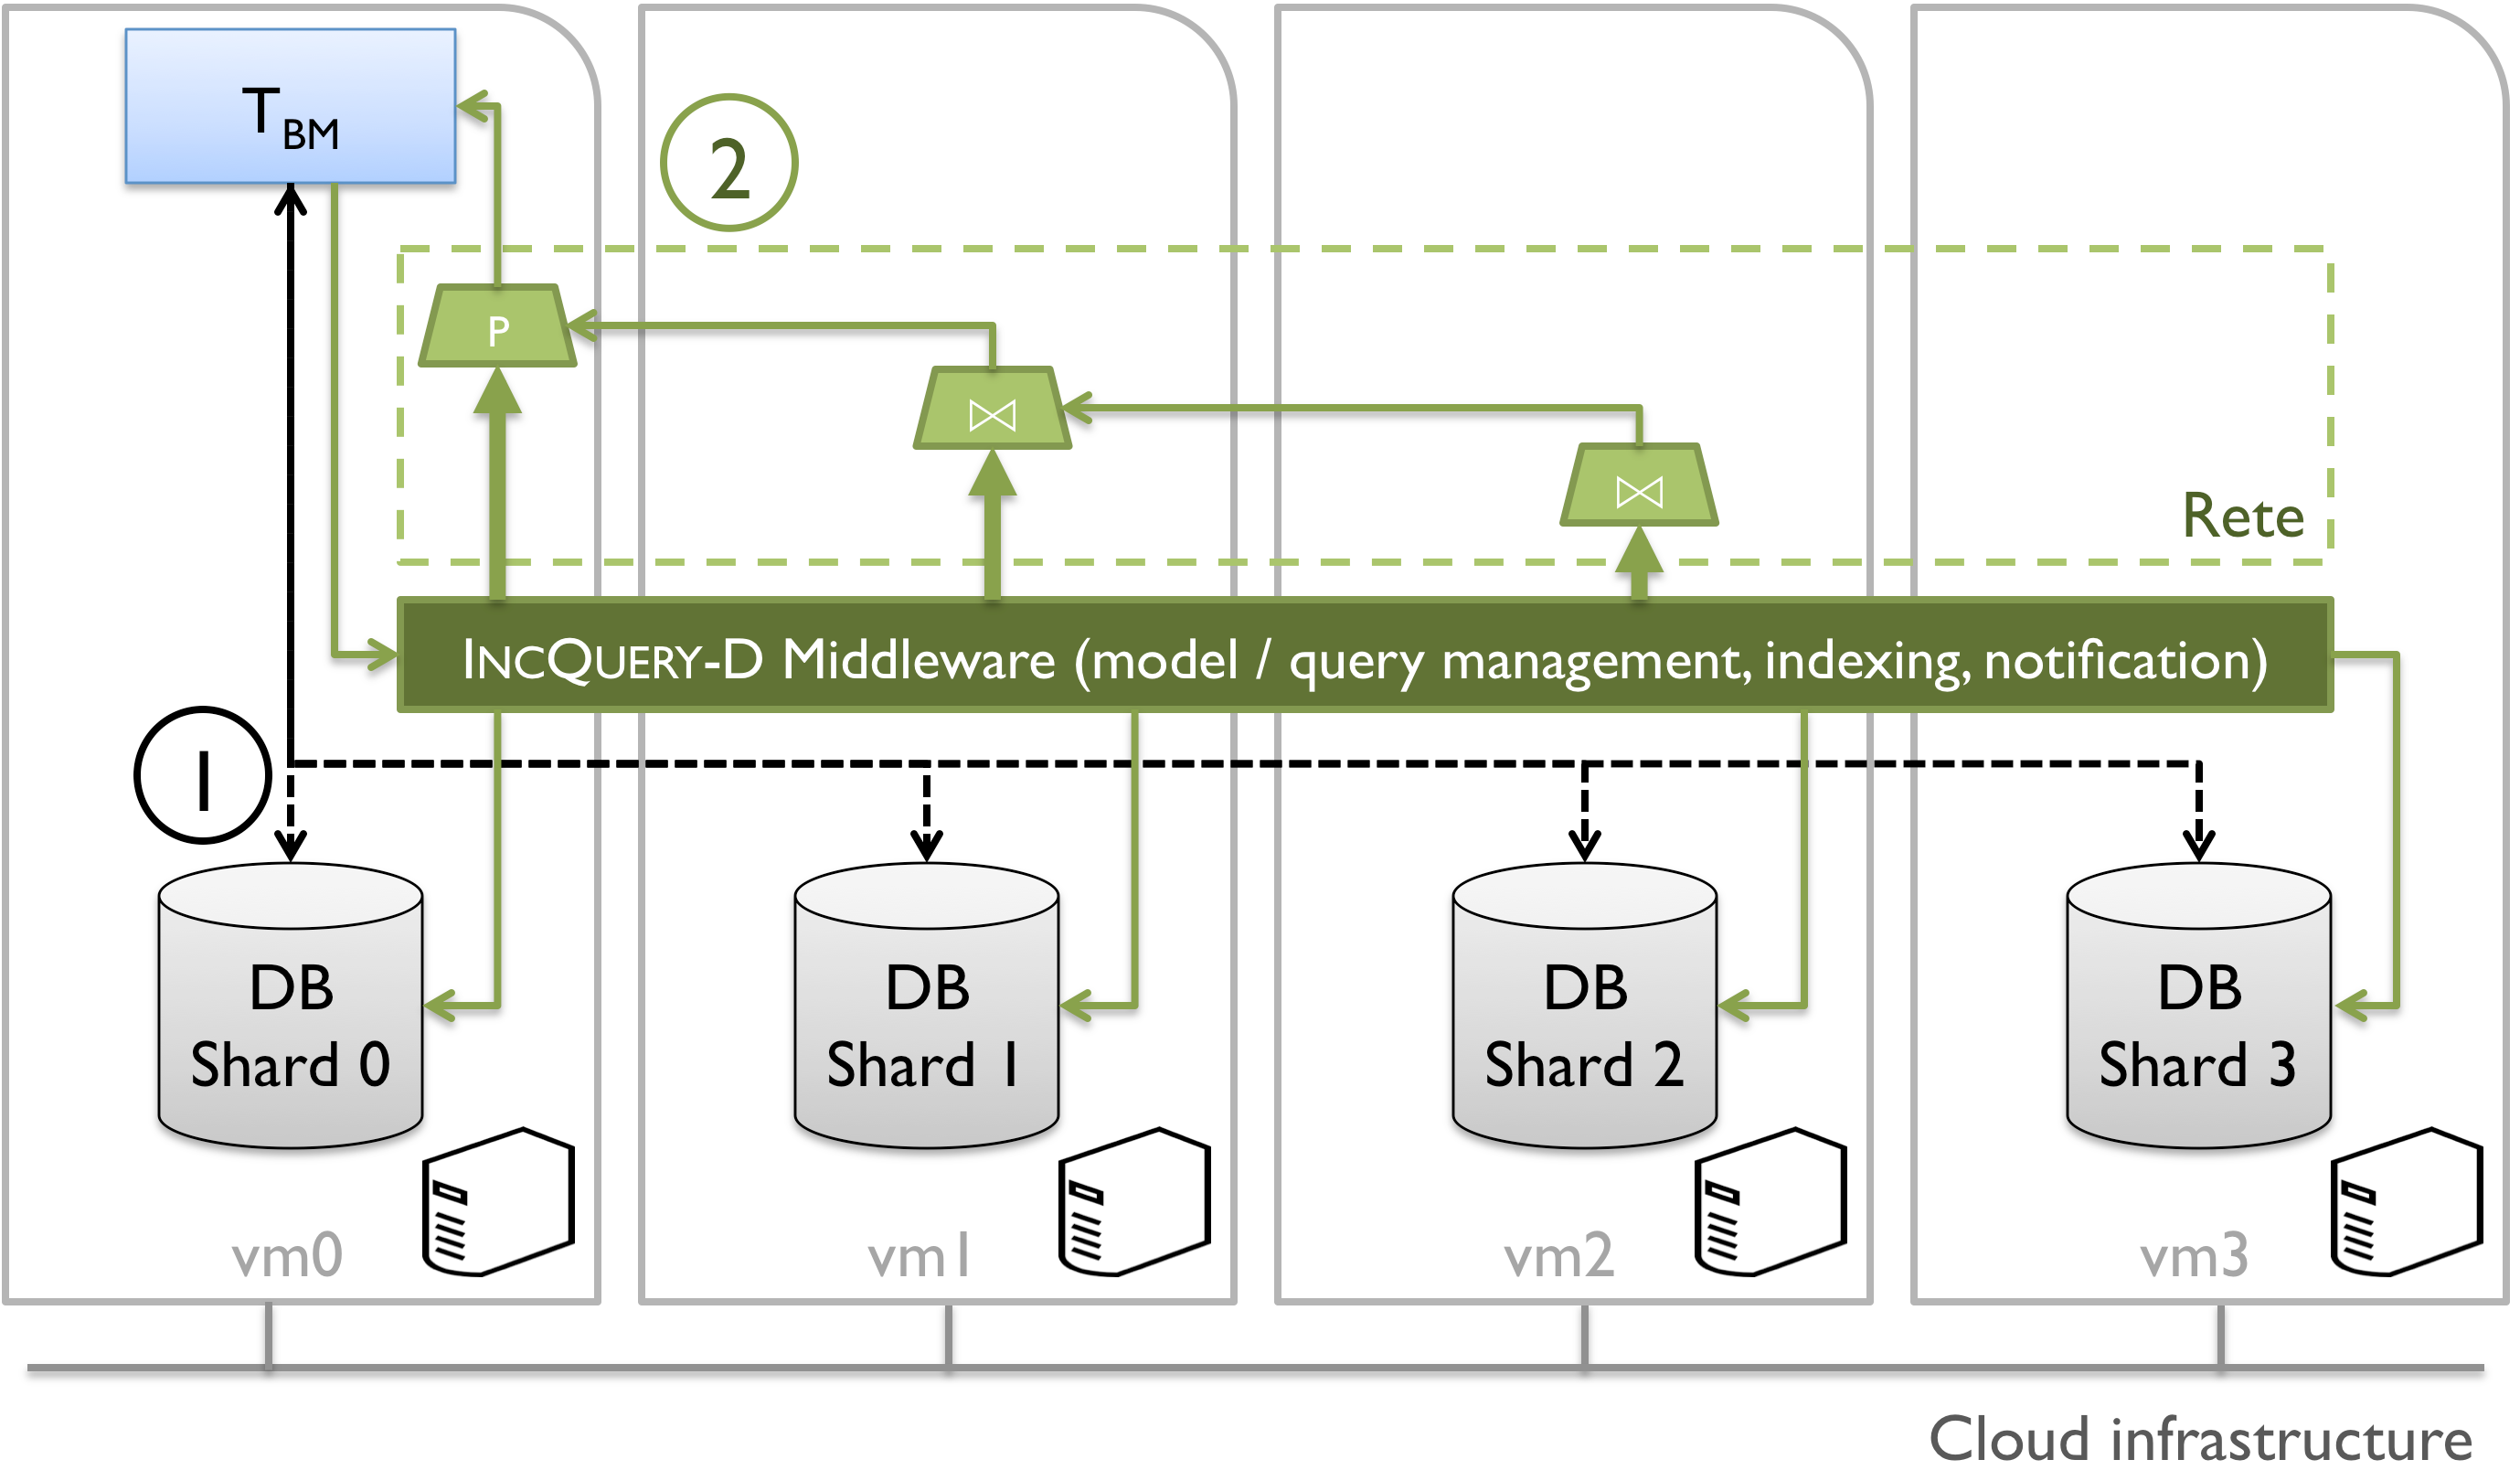
\includegraphics[width=.95\columnwidth]{figures/architecture}
\caption{A distributed, Rete-based model store and query system}
\label{fig:architecture}
\end{center}
\end{figure}


\emph{Storage and middleware.}\label{storage_and_middleware}
The proposed system is based on a distributed database management system.

In recent years, along long standing relational database management systems, dozens of new database systems sprung to life. This systems are often called NoSQL (short for not only SQL) databases.
These systems are often specialized to serve a specific aspect of Web 2.0 applications. To do so, they provide a non-relational data model and weaker consistency guarantees, but offer higher availability and better scalability.

In contrast to a traditional setup, where the distributed model repository (consisting of four shards in the example) is accessed on a per-node basis by a model manipulation transaction (such as a model transformation benchmark, depicted as $T_{BM}$ in \autoref{fig:architecture}), \incqueryD{} provides a middleware layer that offers three core services (shown in green in \autoref{fig:architecture}).
In {{\em distributed model management}}, the primary task is to provide a \emph{surrogate key} mechanism so that each model element in the entire distributed repository can be uniquely identified, and located within storage shards.
{{\em Model indexing}} is the key to high performance model queries. As MDE primarily uses a metamodeling infrastructure, the \incqueryD{} middleware maintains type-instance indexes so that all instances of a given type (both edges and graph nodes) can be enumerated quickly.
Finally, {{\em model change notifications}} are required by incremental query evaluation, thus model changes are captured and their effects propagated in the form of \emph{notification objects} (NOs). The middleware layer achieves this by providing a facade for model manipulation operations. 

Conceptually, the architecture of \incqueryD{} allows the usage of a wide scale of model representation formats. Our first prototype has been evaluated in the context of a low abstraction level \emph{property graph}~\cite{DBLP:journals/corr/abs-1006-2361} data model, but other mainstream metamodeling and knowledge representation languages such as Ecore~\cite{EMF} and RDF~\cite{website:rdf_standard} could be supported, as long as they can be mapped to an efficient and distributed storage backend (like key-value stores or column-family databases).


\emph{Distributed pattern matcher.}\label{distributed_pattern_matcher}
On top of the middleware, \incqueryD{} constructs a distributed and asynchronous network of communicating nodes that implement the Rete~\cite{Forgy} algorithm (shown within the dashed region in \autoref{fig:architecture}). This layer is essentially a dataflow network, with two types of nodes. Change notification objects (tokens) are propagated to intermediate \emph{worker nodes} that perform operations (like filtering tokens based on constant expressions, or performing join or antijoin operations based on their contents) and
store partial (interim) query results in their own memory. In contrast, \emph{production nodes} are terminators that provide an interface for fetching query results and also their changes. Connections between nodes can be \emph{local} (within one host) or \emph{remote} (when two Rete nodes are allocated to different hosts). It is important to emphasize that the database shards and Rete nodes are two distinct levels of distribution that do not directly depend upon each other.

\begin{figure}[!h]
\begin{center}
\begin{tabular}{cc}
\begin{minipage}{0.35\columnwidth}
\begin{lstlisting}
pattern test(
  V1:Type1, V2:Type2,
  V3:Type3, V4:Type4) {
  Type1.edgeType1(V1, V2);
  // join 1
  Type2.edgeType2(V2, V3);
  // join 2
  Type3.edgeType3(V3, V4);
  // antijoin 
  neg find anti(V4, V1); 
}
pattern anti(V4, V1) {
 Type1.edgeType4(V4, V1);
}
\end{lstlisting}
\end{minipage}
\hspace{0.5cm}
\begin{minipage}{0.45\columnwidth}
  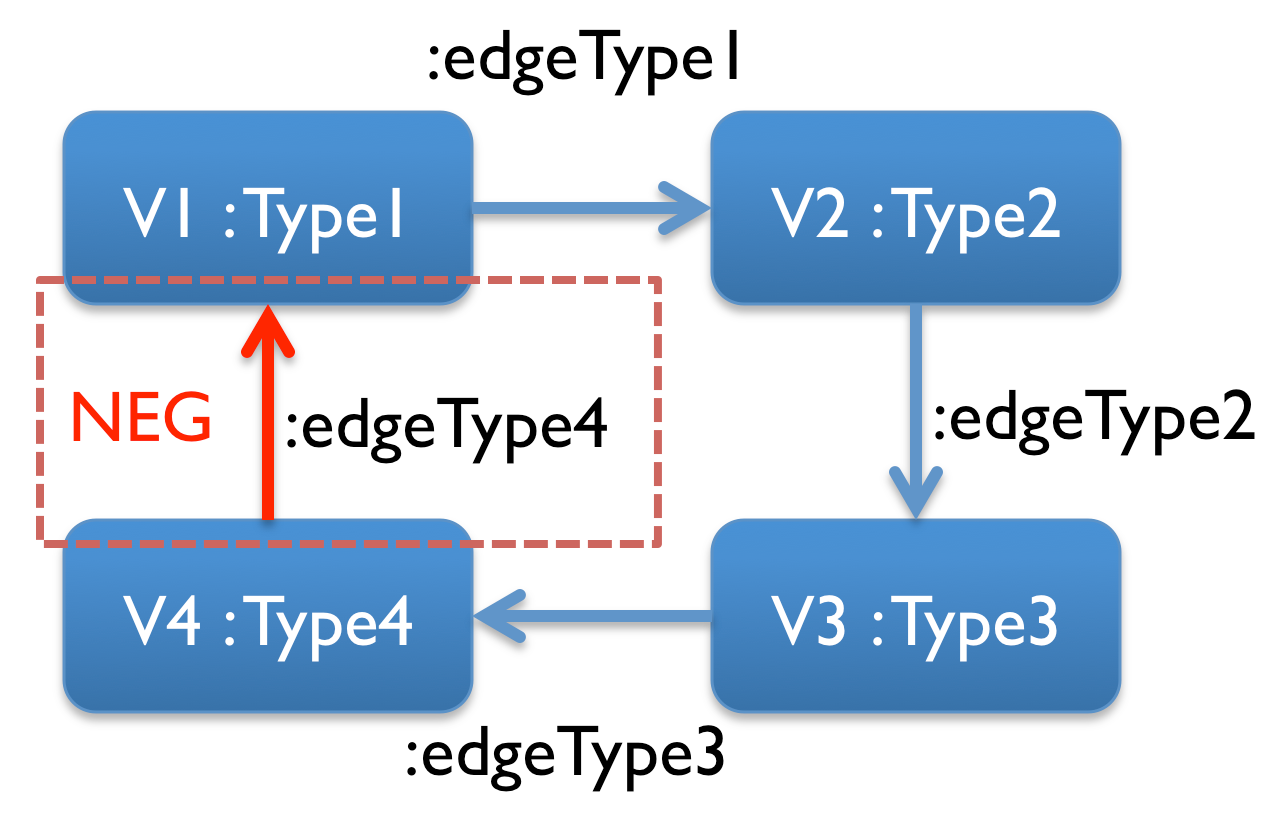
\includegraphics[width=\textwidth]{figures/patterndef}
\end{minipage}
\end{tabular}
\end{center}
\caption{Example graph query}
\label{fig:patterndef}
\end{figure}

\emph{Example.}
An example graph query is shown in \autoref{fig:patterndef} (the query is intentionally domain-independent to emphasize the generalizability of the approach), as a graph pattern definition in \incquery{} syntax~\cite{models10} on the left and graphically on the right. This query represents a typical pattern that is used in MDE applications (such as well-formedness validation or complex model transformations), whereby a subgraph of 4 connected vertices ($V1, V2, V3, V4$) is sought after with a \emph{negative application condition} prescribing that a typed edge (between vertices $V4$ and $V1$) must not exist.
The Rete network constructed for matching this graph pattern is depicted in \autoref{fig:retelayout}. In \incqueryD{}, type-instance indexers for edge types enumerate all source and target vertices, thus the intermediate join nodes perform join operations on vertex pairs that are connected by typed edges as prescribed by the definition in \autoref{fig:patterndef}. The join nodes all store the intermediate query results (e.g.\ connected $V1-V2$ and $V2-V3$ tuples in the case of the leftmost join node), and keep these caches up-to-date as change tokens arrive from the middleware (whenever model changes are performed).

\emph{Information representation and distributed operation.} The Rete layer of \incqueryD{} is \emph{domain and storage agnostic} as it stores only tuples constructed from model element identifiers and literals, thus it can be used independently of the model representation format (metamodeling language) of the model repository.
As illustrated in \autoref{fig:architecture}, the Rete nodes can be allocated to different hosts in a cloud computing infrastructure (as the communication protocol supports remoting). As change propagation is asynchronous, \incqueryD{} implements a \emph{termination protocol} to ensure that the query results can be retrieved consistently with the model state after a given transaction (i.e.\ by signaling when the update propagation has been terminated).

\begin{figure}[!tb]
\begin{center}
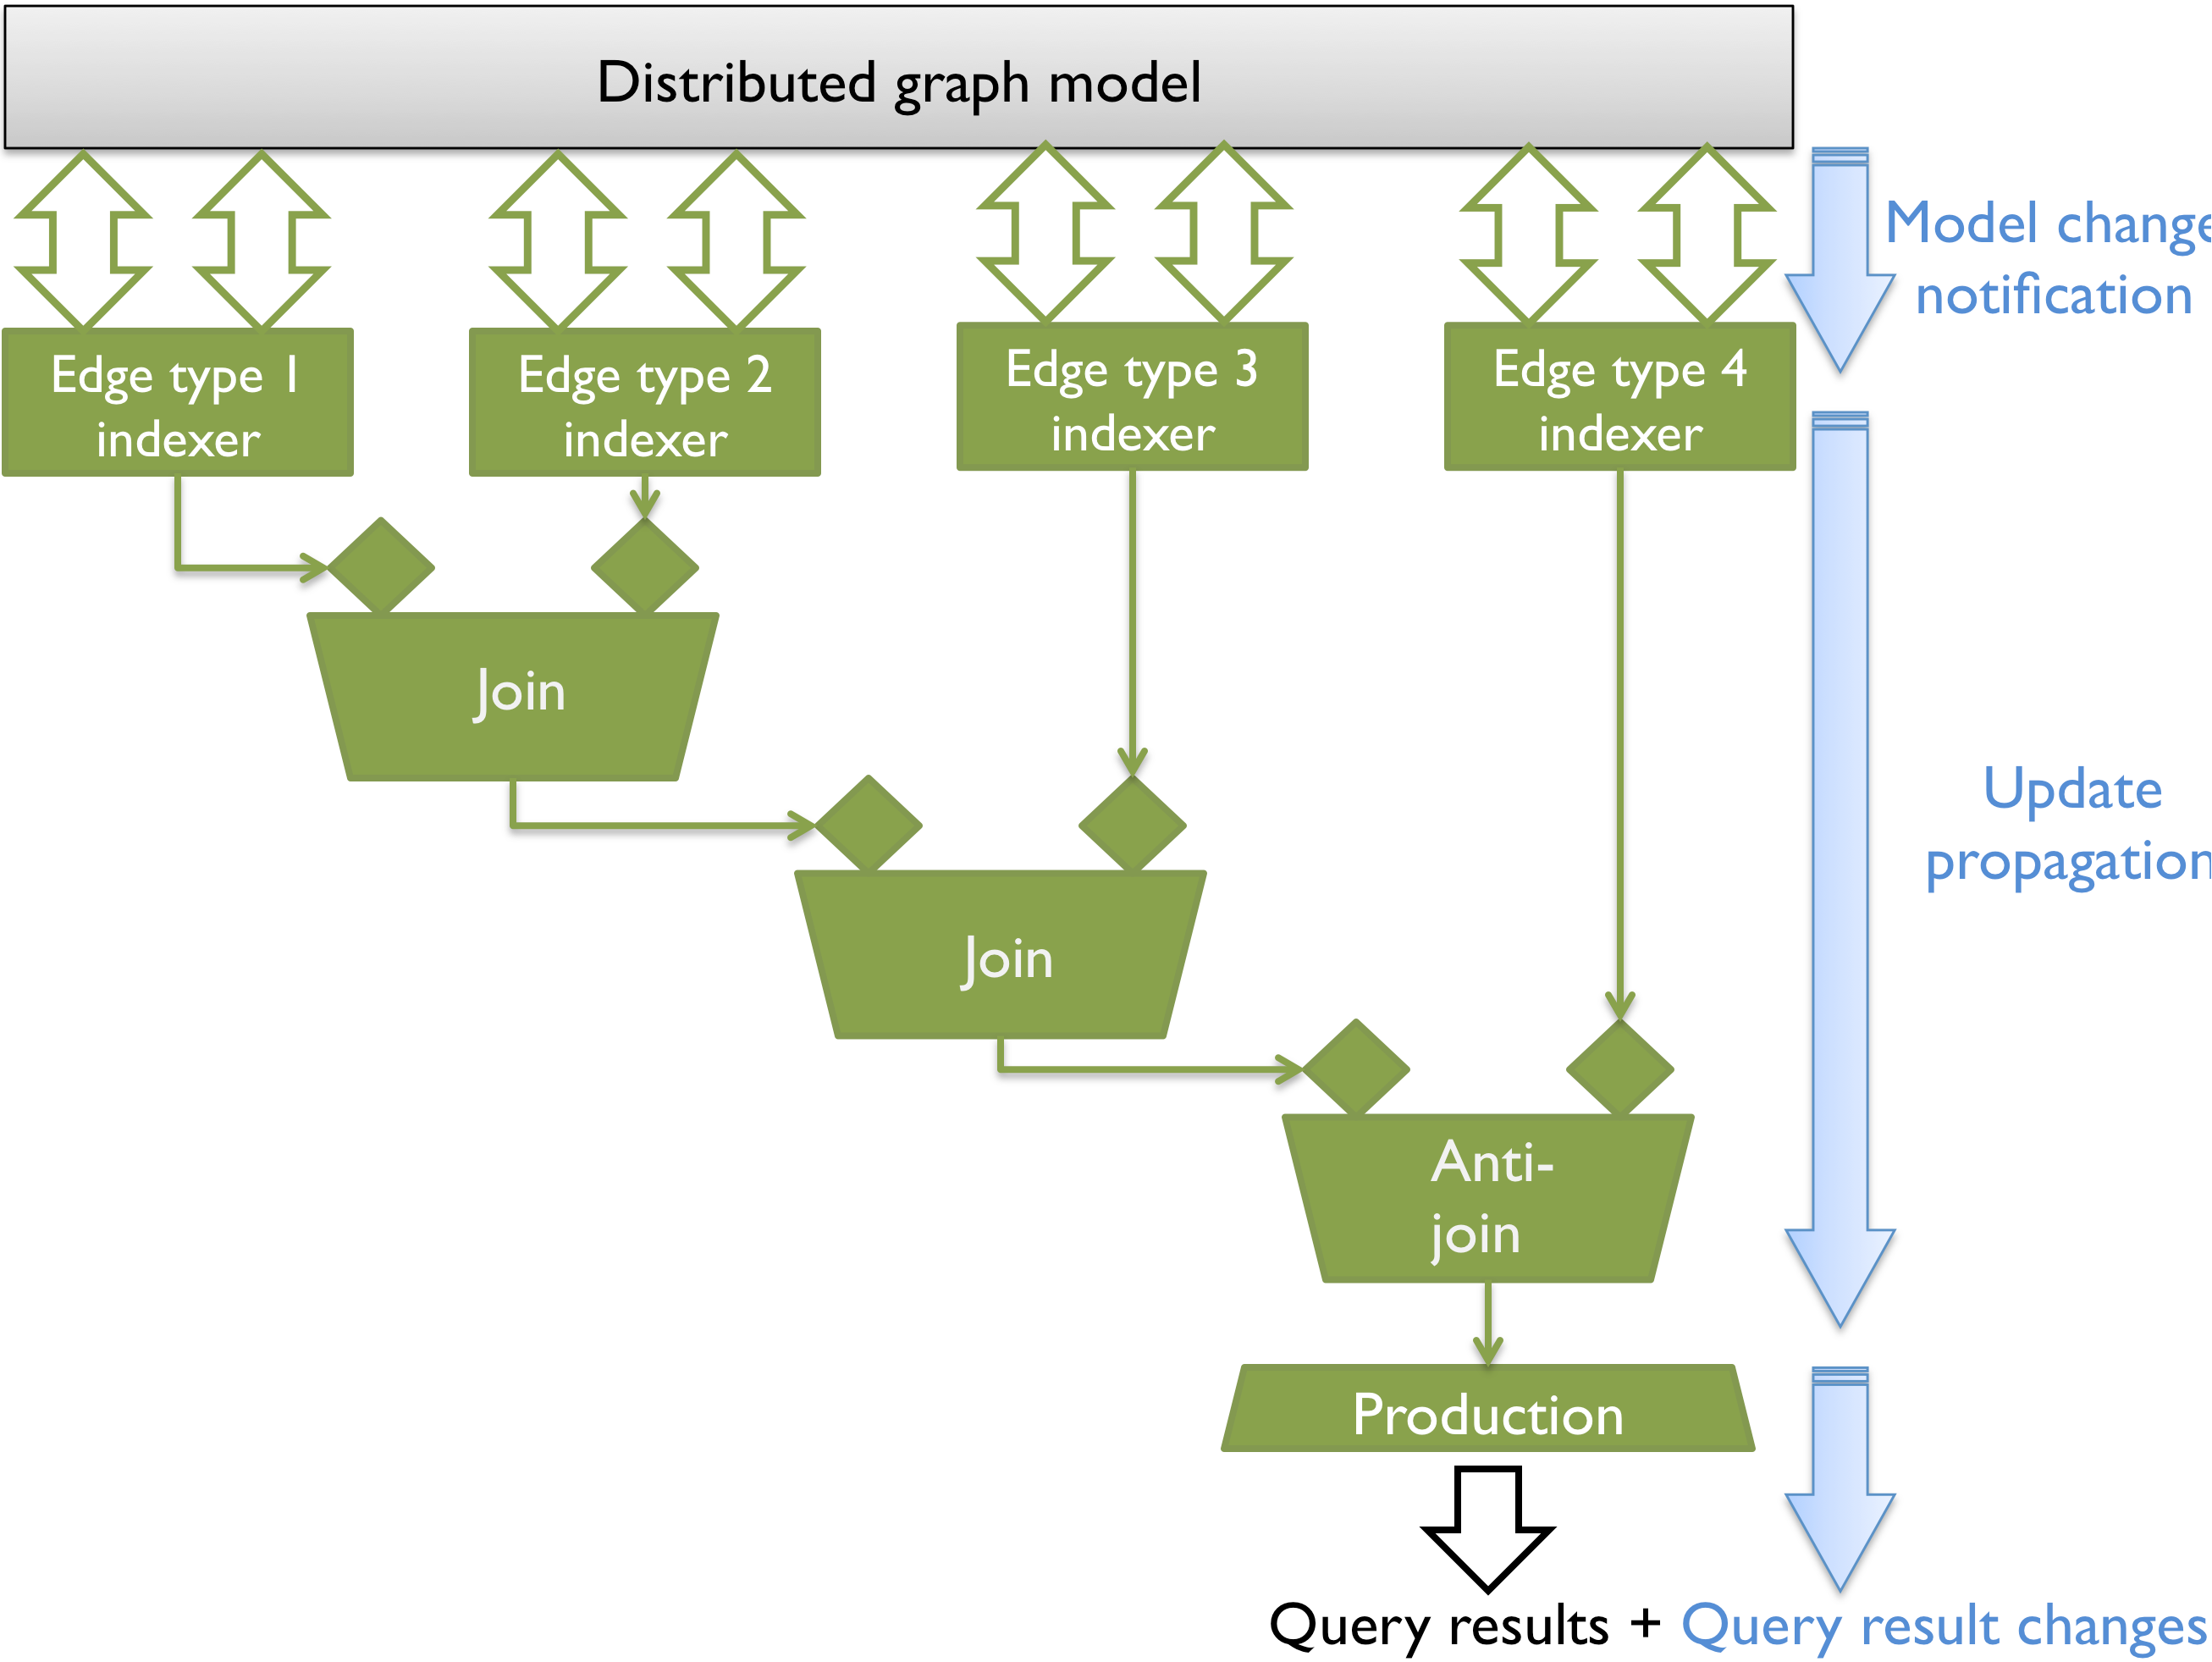
\includegraphics[width=.8\columnwidth]{figures/reteinternals}
\caption{Rete layout}
\label{fig:retelayout}
\end{center}
\end{figure}

\subsection{Scalability considerations}
For the storage layer, the most important issue from an incremental query evaluation perspective is that the indexers of the middleware should be filled as quickly as possible. This favors technologies where model sharding can be performed efficiently (i.e.\ with balanced shards in terms of type-instance relationships), and elementary queries (or model graph traversals) can be executed efficiently.

Achieving scalability of the distributed Rete architecture is an equally complex challenge. The overall performance of the system is influenced by a number of factors, including (i) the \emph{layout of the Rete network} (which can be optimized depending on both query and instance model characteristics, e.g.\ to keep the resource requirement of intermediate join operations to a minimum), (ii) the \emph{allocation} of Rete nodes to host computers (e.g.\ to optimize local resource usage, or to minimize the amount of remote network communication), and (iii) \emph{dynamic adaptability} to changing conditions (e.g.\ when the model size and thus query result size grows rapidly, the Rete network may require dynamic reallocation or node sharding due to local resource limitations).
\chapter{Benchmark}

\section{TrainBenchmark}

The base of my work was a benchmark named \textit{TrainBenchmark} developed by Benedek Izsó, István Ráth and Zoltán Szatmári. The goal of the TrainBenchmark is to compare EMF-IncQuery \cite{incquery} to other (preferably incremental) query tools.

The TrainBenchmark defines two scenarios:

\begin{description}
  \item[UserScenario] This scenario simulates a user sitting in front of her workstation and modifying the model in small steps.
  \item[XFormScenario] This scenario simulates a software running automated transformations on the model.
\end{description}

\subsection{Metamodel}

TrainBenchmark works on a railroad's model. The metamodel is shown on \autoref{fig:metamodel}.

\begin{figure}
\begin{center}
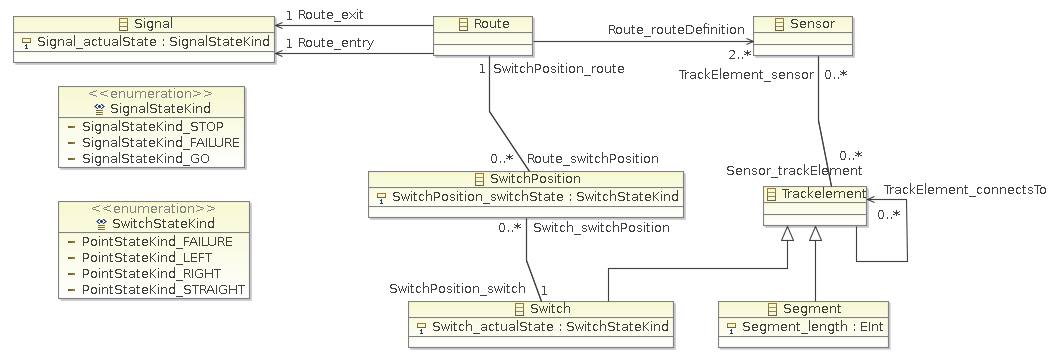
\includegraphics[width=14cm]{figures/TrainMetamodel}
\caption{The metamodel for the TrainBenchmark}
\label{fig:metamodel}
\end{center}
\end{figure}

The \texttt{generator} project of TrainBenchmark is capable of generating railroad instance models of different sizes. The project contains classes for generating models in different formats, including EMF, OWL, RDF and SQL.

\section{Queries}

The queries in TrainBenchmark look for violations of well-formedness constraints in the model. We only discuss the \textit{RouteSensor} query in detail.

\subsection{RouteSensor}

The \textit{RouteSensor} query looks for \textit{Sensors} that are connected to a \textit{Switch}, but the sensor and the switch are \textit{not} connected to the same \textit{Route}. The graphical representation of the RouteSensor query is shown on \autoref{fig:routesensor}.

\begin{figure}
\begin{center}
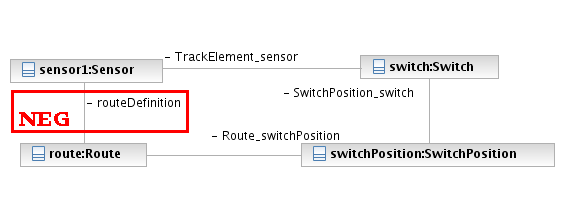
\includegraphics[]{figures/OD_RouteSensor}
\caption{Graphical representation of the RouteSensor query}
\label{fig:routesensor}
\end{center}
\end{figure}

The Cypher code for all TrainBenchmark queries is shown in detail in \autoref{cypherqueries}.

\section{Phases}

The TrainBenchmark consists of the following phases:

\begin{enumerate}
  \item $read$: loading the model,
  \item $check_0$: running the queries,
  \item $edit_i$: editing the model, 
  \item $check_i$: running the queries again.
\end{enumerate}

In a ,,real-world'' model editing sequence, the user tipically edits the model in small steps ($edit_i$ phases). The user's work is much more productive if she receives an instant feedback, hence we would like to run re-evaluate well-formedness queries quickly (preferably in sub-second time). This creates the need for an incremental pattern matcher tools.

\section{Neo4j}

NoSQL database management system come in many flavor, including \textit{graph databases} \cite{NoSQL}. Neo4j is the most popular and most funded graph database on the market today. Neo4j is developed by a Swedish company Neo Technology since 2002 \cite{neo4j}. It's available as an open source project since 2007.

\begin{figure}
\begin{center}

\includegraphics[]{figures/neo4j-logo}
\caption{The logo of Neo4j}
\label{fig:neo4j-logo}
\end{center}
\end{figure}

Neo4j graphs can be visualised in Neoclipse, an Eclipse RCP application \cite{Neoclipse}.

\begin{figure}
\begin{center}
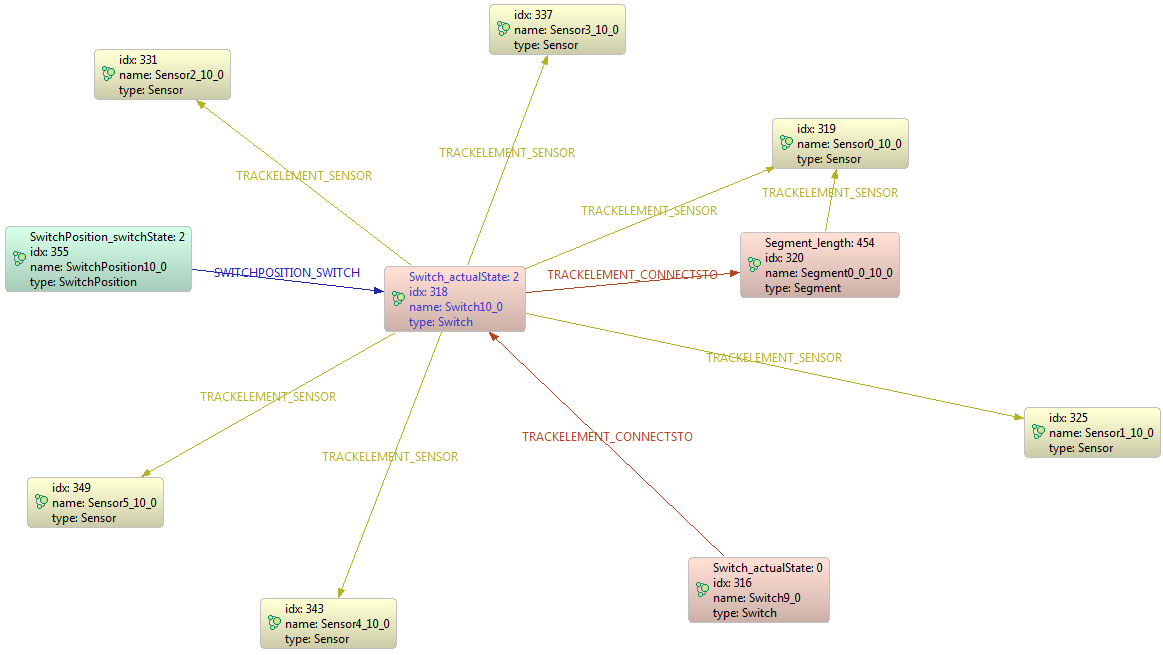
\includegraphics[width=14cm]{figures/neoclipse-graph}
\caption{A subgraph of a TrainBenchmark instance visualised in Neoclipse}
\label{fig:neoclipse}
\end{center}
\end{figure}

The lack of a common formal data model is both an advantage and a shortcoming of NoSQL databases. The Tinkerpop framework \cite{Tinkerpop} aims to provide a common data model and interface for graph databases.

\section{Generation of models}

I created a property graph generator project based on the previous TrainBenchmark generators. The generator creates a graph in an embedded Neo4j database and uses the Blueprints library's \texttt{GraphMLWriter} class to save to a GraphML file \cite{Blueprints}.

\subsection{RouteSensor}

The Cypher implementation of the RouteSensor query is shown on \autoref{lst:cypher-routesensor}

\begin{lstlisting}[caption=Cyper query for the RouteSensor test case, label=lst:cypher-routesensor, breaklines=true]
START sensor=node:node_auto_index(type="Sensor")
MATCH sensor-[:TRACKELEMENT_SENSOR]-switch-[:SWITCHPOSITION_SWITCH]-switchPosition-[:ROUTE_SWITCHPOSITION]-route-[r?:ROUTE_ROUTEDEFINITION]-sensor
WHERE r IS NULL
RETURN sensor
\end{lstlisting}

\chapter{Evaluation}
\label{sec:evaluation}

% 1 hasab + 1 abra helyed van, helytakarekosan irj, keruld az itemize-okat

We implemented \iqd{} as an initial prototype to evaluate the feasibility of the approach, and to experiment with various optimization possibilities. As the storage, we used the popular graph database Neo4j \cite{neo4j} featuring automatic indexes and two core query technologies (Gremlin and Cypher) that were used as a low-level model access interface by our middleware layer. % TODO middleware: blueprints, but custom implementation because\ldots
The prototype of the distributed middleware and Rete network were implemented in Java using Akka~\cite{akka}, the Scala-based toolkit for building applications based on the Actor model, since it is well-suited for asynchronous applications. The communication protocol was built on top of Akka's built-in serialization support.


%TODO mit merunk? model manipulacios muveletek es query kiertekeles valaszido
%adott: query def, modell manipulacios szekvencia

% 4 fazisban az alabbiak szerint TODO
%generalt: novekvo meretu modellek (hogyan generaltuk, mi a query-k eredmenyhalmaz meretenek viszonya a modellhez?, 

%mi az elosztott modell sajatossaga/limitacioja (nincsenek keresztelek))

%mert: lekerdezesek, ill. manip. tranzakcio lefutasi ideje

\section{Benchmark scenario}

\label{benchmark}
In order to measure the efficiency of model queries and manipulation operations over the distributed architecture, we designed a benchmark to measure tool response times in a well-formedness validation use case. The benchmark transaction sequence consists of four phases: (i) during the $load$ phase, the serialization of the model is loaded into the database; (ii) a test query (\autoref{fig:patterndef}) is executed ($check_0$); finally, in a cycle consisting of several repetitions, some elements are programmatically modified ($edit_i$) and the test query is re-evaluated ($check_i$). We ran the benchmark on pseudo-randomly generated instance models of growing size, each model containing about twice as many elements (vertices and edges) as the previous one and having a regular fan-out structure. As the current version of Neo4j does not have built-in support for graph sharding, the benchmark uses a manually sharded strategy where each shard contains a disjoint partition of the model.


%TODO referencia leirasa (miert az, ami?)
% We implemented two approaches
% on top of Neo4j.
% Non-incremental: uses only Cypher for the pattern matching. 
%   Beside Neo4j's indexes, no additonal data structures are built.

% TODO sajat implementacio leirasa (manualis allokacio)

% Incremental: builds a distributed Rete network to support incremental pattern matching, and 
%     maintains both the databases and the Rete net upon modification. 
%     Only uses Cypher to retrieve the graph nodes for the type indexers of the Rete net. 

% For the incremental query, we manually created the Rete network and 
% generated random instance models of different sizes to benchmark the query's execution time.

\label{benchmark_environment}
\section{Evaluation aspects and benchmark environment}

To compare the performance characteristics of \iqd{} to a traditional case, we defined two scenarios. The \textit{batch} scenario uses only Neo4j to manage models and evaluate the queries in a parallelized way (depicted as \textcircled{1} in \autoref{fig:architecture}). This serves as a baseline for the \textit{incremental} scenario, which uses \iqd{} (shown as \textcircled{2} in \autoref{fig:architecture}). For these initial experiments, the layout and allocation of the Rete network was determined manually. As the testbed, we deployed our system to a private cloud consisting of 4 virtual machines on separate host computers. Each virtual machine used dual 2.5 GHz Intel Xeon L5420 CPUs with 16 GBs of RAM, running on Ubuntu 12.10 64 bit with Neo4j 1.8 and Akka 2.1.2. More details are available at \url{http://incquery.net/publications/trainbenchmark}.

\begin{figure}
\begin{center}
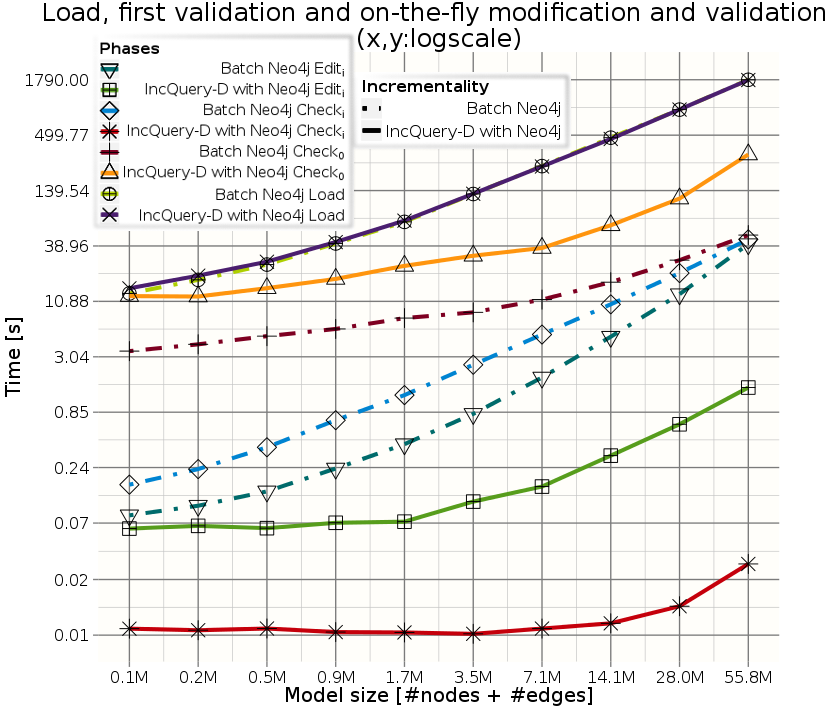
\includegraphics[width=\columnwidth]{figures/All_RouteSensor}
\caption{Benchmark results}
\label{fig:benchmark}
\end{center}
\end{figure}

\section{Results}
\label{benchmark_results}\label{analysis}

The measurement results of our experiments are shown in \autoref{fig:benchmark} (aggregated from several complete sets to filter transient effects). As expected, the $load$ phase take about the same time for both scenarios, and \iqd{} is about half an order of magnitude slower when evaluating the query at first (\textit{check 0} phase) due to the Rete construction overhead. However, \iqd{} is several orders of magnitude faster during the $edit_i - check_i$ cycles, making on-the-fly query (re)evaluation feasible even for models larger than 50 million elements. Once initialized, \iqd{} scales linearly, since query response times for growing models can be kept low by adding additional computers for hosting Rete nodes.

The Rete implementation is based on the Rete algorithm, originally created by Charles Forgy \cite{Forgy} and improved by Gábor Bergmann \cite{BergmannRete}.

\section{Technologies}

\subsection{Akka}

Akka is a toolkit and runtime for building highly concurrent, distributed, and fault tolerant event-driven applications on the JVM \cite{akka}. In my implementation, the remote nodes run on Akka \textit{microkernels}. The actors are instantiated using the \textit{remote deployment} feature.

\begin{figure}
\begin{center}

\includegraphics[width=6cm]{figures/akka-logo}
\caption{The logo of Akka}
\label{fig:akka-logo}
\end{center}
\end{figure}

The alpha nodes (called \textit{UniquenessEnforcerNodes}) store the edges and their source and destination nodes in their memory.

Currently, these graph elements are retrieved by Cypher (\autoref{lst:cypher-route-routedefinition}).

\begin{lstlisting}[caption=Cypher query to retrieve all \texttt{ROUTE\_ROUTEDEFINITION} edges, label=lst:cypher-route-routedefinition, breaklines=true]
START
    route=node:node_auto_index(type='Route'),
    sensor=node:node_auto_index(type='Sensor')
MATCH (route)-[:ROUTE_ROUTEDEFINITION]->(sensor)
RETURN route.idx AS routeId, sensor.idx AS sensorId;
\end{lstlisting}

\subsection{Google Guava}

The implementation relied heavily on Google Guava library's Collections framework \cite{guava}. The Guava Collection is an extension to Java's Collection framework. We used immutable collections and new type of collections (e.g.\ Multimap).

\subsection{Neo4j Java REST binding}

I used Neo4j in \textit{server mode} and accessed the REST interface with the \texttt{java-rest-binding} library \cite{restbinding}.

\subsection{Apache Maven}

To integrate the technologies, we used Apache Maven \cite{Maven}, an open source build automation system.

\chapter{Related and future work}



\section{Related work}
\label{sec:relwork}

A wide range of special languages have been developed to support \emph{graph based} representation and querying of computer data. A class-diagram like modeling language is Ecore of the Eclipse Modeling Framework (EMF~\cite{EMF}), where classes, references between them and attributes of classes describe the domain. Extensive tooling helps the creation and transformation of such domain models. For EMF models, OCL is a declarative constraint description and query language that can be evaluated with the local-search based Eclipse OCL~\cite{EclipseOCL} engine. To address scalability issues, impact analysis tools~\cite{OCLIA} have been developed as extensions or alternatives to Eclipse OCL.

Outside the Eclipse ecosystem, the Resource Description Framework (RDF~\cite{website:rdf_standard}) is developed to support the description of instances of the semantic web, assuming sparse, ever-growing, incomplete data. Semantic models are built up from triple statements and they can be queried using the SPARQL~\cite{SPARQL} graph pattern language with tools like Sesame~\cite{sesame} or Virtuoso~\cite{openvirtuoso}. Property graphs~\cite{DBLP:journals/corr/abs-1006-2361} provide a more general way to describe graphs by annotating vertices and edges with key-value properties. Such data structures can be stored in graph databases like Neo4j~\cite{neo4j} which provides the Cypher~\cite{cypher} query language. Even though big data storage (usually based on MapReduce) provides fast object persistence and retrieval, query engines realized directly on these data structures do not provide dedicated support for incremental query evaluation. 

In the context of event-based systems, distributed evaluation engines were proposed earlier~\cite{message-passing-rete}. However they scaled up in the number of rules \cite{mapreduce-rete} rather than in the number of data elements. As a very recent development, Rete-based caching approaches have been proposed for the processing of Linked Data (bearing the closest similarity of our approach). INSTANS~\cite{INSTANS2012} uses this algorithm to perform complex event processing (formulated in SPARQL) on RDF data, gathered from distributed sensors. Diamond~\cite{miranker2012diamond} evaluates SPARQL queries on Linked Data, but it lacks an indexing middleware layer so their main challenge is efficient data traversal.

The conceptual foundations of our approach as based on \eiq{}~\cite{models10}, a tool that evaluates graph patterns over EMF models using Rete. Up to our best knowledge, \iqd{} is the first approach to promote distributed scalability by \emph{distributed incremental query evaluation} in the MDE context. As the architecture of \iqd{} separates the data store from the query engine, we believe that the scalable processing of property graphs can open up interesting applications outside of the MDE world.


Acharya et al. described a Rete network mapping for fine grained and medium grained message-passing computers~\cite{message-passing-rete}. The medium-grained computer connected processors in a crossbar architecture, while our approach use computers connected by gigabit ethernet. The paper published benchmark results of the medium-grained solution, but these are based only on simulations.

\section{Future work}

\subsection{Cassandra}

Apache Cassandra is a mature, popular NoSQL database that stores \textit{column families} \cite{Cassandra}. Column families are similar to tables in relational databases, but have a looser schema: each row has it's set of columns.

Cassandra is fault-tolerant and highly scalable with tunable consistency properties. It's distributes the rows in the cluster using a \textit{partitioner}.

\begin{figure}
\begin{center}

\includegraphics[]{figures/cassandra-logo}
\caption{The logo of Cassandra}
\label{fig:cassandra-logo}
\end{center}
\end{figure}


\subsection{Clustered graph loader application}

The \textit{ClusterGraphLoader} application is capable of bulk loading a graph (stored in a GraphML file) to a Cassandra cluster.

The GraphML file is stored on a distributed file system, currently HDFS \cite{hadoop}. The parsing of the GraphML file is divided to to phases:

\begin{enumerate}
  \item Scan the file to determine the \texttt{<node>} and \texttt{<edge>} segments.
  \item Parse the file parallelly.
\end{enumerate}

For the second phase, we implemented a sequential GraphML parser using the Woodstox XML parser library \cite{Woodstox} which overrides the JDK's default StAX parser (\texttt{javax.xml.stream}). The second phase runs distributedly in the cluster using Akka actors and loads the nodes and edges to the Cassandra cluster. 

\subsection{Titan}

Titan is a highly scalable graph database optimized for storing and querying large graphs with billions of vertices and edges distributed across a multi-machine cluster \cite{Titan, TitanRiseOfBigData, TitanCassandra}.

Titan supports various storage backends, including Apache Cassandra \cite{Cassandra} and Apache HBase \cite{HBase}. Unlike disk-based graph databases (e.g.\ Neo4j), Titan offers horizontal scalability and sharding of graphs.

\begin{figure}
\begin{center}

\includegraphics[]{figures/titan-logo}
\caption{The logo of Titan}
\label{fig:titan-logo}
\end{center}
\end{figure}

For our experiments, we used Cassandra as the storage backend because of it's easy deployment and great tunability.

\subsubsection{Titan and Cassandra setups}

In order to use Gremlin's full processing power, we have to use Rexster, a graph server that exposes any Blueprints graph through REST \cite{Rexster}.

Titan, Cassandra and Rexster can be deployed in two different setups: remote server mode(\autoref{fig:titan-modes-rexster}) and the embedded mode (\autoref{fig:titan-modes-embedded}).

\begin{figure}
\begin{center}
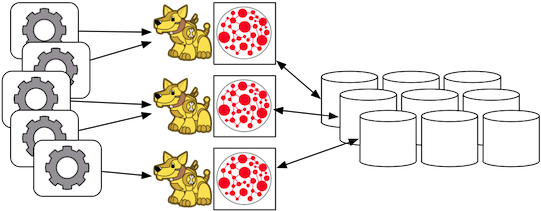
\includegraphics[width=10cm]{figures/titan-modes-rexster}
\caption{Titan's remote server mode}
\label{fig:titan-modes-rexster}
\end{center}
\end{figure}

\begin{figure}
\begin{center}
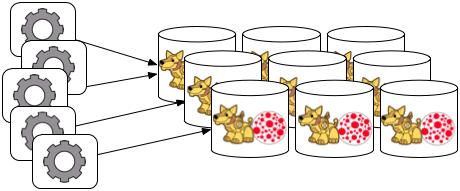
\includegraphics[width=10cm]{figures/titan-modes-embedded}
\caption{Titan's embedded mode}
\label{fig:titan-modes-embedded}
\end{center}
\end{figure}

\subsubsection{Initialising Titan}

\begin{lstlisting}[caption=Gremlin commands to initialize the a single-node Titan instance, label=lst:titan-singlenode, breaklines=true]
g = TitanFactory.open('mygraphdir');
g.createKeyIndex("idx", Vertex.class);
g.createKeyIndex("type", Vertex.class);
g.loadGraphML('/home/szarnyasg/data/testBig_User_1.graphml');
\end{lstlisting}

\subsubsection{Listing nodes}

The Gremlin code to list all \texttt{ROUTE\_ROUTEDEFINITION} edges is shown in \autoref{lst:gremlin-route-routedefinition} (see also the Cypher query in \autoref{lst:cypher-route-routedefinition})

\begin{figure}
\begin{center}

\includegraphics[]{figures/gremlin-logo}
\caption{The logo of Gremlin}
\label{fig:gremlin-logo}
\end{center}
\end{figure}

\begin{lstlisting}[caption=Gremlin query to retrieve all \texttt{ROUTE\_ROUTEDEFINITION} edges, label=lst:gremlin-route-routedefinition, breaklines=true]
t = new Table(); 
g.idx('node_auto_index')[[type:'Route']].as('Route').outE('ROUTE_ROUTEDEFINITION').as('RouteDefinition').inV.as('Sensor').table(t).iterate();
t;
\end{lstlisting}

\chapter{Conclusion}
\label{sec:conclusion}

We presented \incqueryD{}, a novel approach to adapt distributed incremental query techniques to large and complex model driven software engineering scenarios. Our proposal is based on a distributed Rete network that is decoupled from sharded graph databases by a middleware layer, and its feasibility has been evaluated using a benchmarking scenario of on-the-fly well-formedness validation of software design models. The results are promising as they show nearly instantaneous query re-evaluation as model sizes grow well beyond $10^7$ elements.
For future work, we plan on providing more sophisticated automation for sharded Ecore models, and further exploring advanced optimization challenges such as dynamic reconfiguration and fault tolerance.
We also plan experiment with programming languages that are better suited to asynchronous algorithms (e.g.\ Erlang and Scala) and try different database systems (e.g. 10gen MongoDB) as our storage layer.


\addcontentsline{toc}{chapter}{Bibliography} % Add bibliography
\bibliographystyle{plain}                    % use plain style
\bibliography{bib}             % include the entries

\appendix

\chapter{Property graph formats}

%\section{Property graph formats}
\label{sec:property-graph-formats}

In this section, we provide examples for the different property graph formats. The examples describe a small instance model based on the \tb{}'s metamodel, shown on \figref{trainbenchmark-instancemodel-subgraph}.

\myFigureSmall{trainbenchmark-instancemodel-subgraph}{An example graph based on the \tb{}'s metamodel}

%\subsection{GraphML}
\section{GraphML}

%     <node id="0">
%       <data key="type">root</data>
%     </node>
\lstset{language=XML,breaklines=true}
\begin{lstlisting}[caption=A graph based on the \tb{}'s metamodel stored in \graphml{} format]
<?xml version="1.0" encoding="UTF-8"?>
<graphml xmlns="http://graphml.graphdrawing.org/xmlns" xmlns:xsi="http://www.w3.org/2001/XMLSchema-instance" xsi:schemaLocation="http://graphml.graphdrawing.org/xmlns http://graphml.graphdrawing.org/xmlns/1.1/graphml.xsd">
  <key id="id" for="node" attr.name="id" attr.type="int" />
  <key id="type" for="node" attr.name="type" attr.type="string" />
  <graph id="G" edgedefault="directed">
    <node id="1">
      <data key="id">0</data>
      <data key="type">Sensor</data>
    </node>
    <node id="2">
      <data key="id">1</data>
      <data key="type">Route</data>
    </node>
    <node id="3">
      <data key="id">2</data>
      <data key="type">SwitchPosition</data>
    </node>
    <node id="4">
      <data key="id">3</data>
      <data key="type">Switch</data>
    </node>
    <edge id="0" source="2" target="1" label="ROUTE_ROUTEDEFINITION" />
    <edge id="1" source="2" target="3" label="ROUTE_SWITCHPOSITION" />
    <edge id="2" source="3" target="4" label="SWITCHPOSITION_SWITCH" />
    <edge id="3" source="4" target="1" label="TRACKELEMENT_SENSOR" />
  </graph>
</graphml>
\end{lstlisting}

%\subsection{Blueprints GraphSON}
\section{Blueprints GraphSON}

%     {
%       "type":"root",
%       "_id":0,
%       "_type":"vertex"
%     },
%  "mode":"NORMAL",
\lstset{language=json,firstnumber=1}
\begin{lstlisting}[caption=A graph based on the \tb{}'s metamodel stored in Blueprints \graphson{} format]
{
  "vertices":[
    {
      "id":0,
      "type":"Sensor",
      "_id":1,
      "_type":"vertex"
    },
    {
      "id":1,
      "type":"Route",
      "_id":2,
      "_type":"vertex"
    },
    {
      "id":2,
      "type":"SwitchPosition",
      "_id":3,
      "_type":"vertex"
    },
    {
      "id":3,
      "type":"Switch",
      "_id":4,
      "_type":"vertex"
    }
  ],
  "edges":[
    {
      "_id":0,
      "_type":"edge",
      "_outV":2,
      "_inV":1,
      "_label":"ROUTE_ROUTEDEFINITION"
    },
    {
      "_id":1,
      "_type":"edge",
      "_outV":2,
      "_inV":3,
      "_label":"ROUTE_SWITCHPOSITION"
    },
    {
      "_id":2,
      "_type":"edge",
      "_outV":3,
      "_inV":4,
      "_label":"SWITCHPOSITION_SWITCH"
    },
    {
      "_id":3,
      "_type":"edge",
      "_outV":4,
      "_inV":1,
      "_label":"TRACKELEMENT_SENSOR"
    }
  ]
}
\end{lstlisting}

%\subsection{Faunus GraphSON}
\section{Faunus GraphSON}

%{"type":"root","_id":0,"_outE":[],"_inE":[]}
\begin{lstlisting}[caption=A graph based on the \tb{}'s metamodel stored in Faunus \graphson{} format]
{"id":0,"type":"Sensor","_id":1,"_outE":[],"_inE":[{"_id":0,"_outV":2,"_label":"ROUTE_ROUTEDEFINITION"},{"_id":3,"_outV":4,"_label":"TRACKELEMENT_SENSOR"}]}
{"id":1,"type":"Route","_id":2,"_outE":[{"_id":0,"_inV":1,"_label":"ROUTE_ROUTEDEFINITION"},{"_id":1,"_inV":3,"_label":"ROUTE_SWITCHPOSITION"}],"_inE":[]}
{"id":2,"type":"SwitchPosition","_id":3,"_outE":[{"_id":2,"_inV":4,"_label":"SWITCHPOSITION_SWITCH"}],"_inE":[{"_id":1,"_outV":2,"_label":"ROUTE_SWITCHPOSITION"}]}
{"id":3,"type":"Switch","_id":4,"_outE":[{"_id":3,"_inV":1,"_label":"TRACKELEMENT_SENSOR"}],"_inE":[{"_id":2,"_outV":3,"_label":"SWITCHPOSITION_SWITCH"}]}
\end{lstlisting}

\label{page:last}
\end{document}
